% Chapter 5

\chapter{High-dimensional inference of mutual information} % Main chapter title

\label{Chapter5} % For referencing the chapter elsewhere, use \ref{Chapter1} 

\section{Motivation}

In the previous chapter, we saw that the identification accuracy of
predicting $Y$ given $X$ can be used to yield a lower bound on
$\text{I}(X; Y)$.  This relied on the inequality relating $k$-class
average Bayes accuracy and mutual information.  However, because in
some cases the mutual information may be much higher than the lower
bound, the estimator $\hat{I}_{Ident}$ may remain an underestimate of
mutual information, even under favorable sample size conditions.  In
other words, the estimator $\hat{I}_{Ident}$ is not consistent.  On the
other hand, the theory behind $\hat{I}_{Ident}$ relies on extremely weak
assumptions.  This makes the estimator quite generally applicable, but
on the other hand, much better estimators may be available in certain
applications where much stronger assumptions can be made.

In this chapter we develop yet another estimator of mutual information
based on identification accuracy, but this time making relatively strong
assumptions relating to the dimensionality of the data and the
dependence structure of the components.  As we will spell out in more
detail in section \ref{sec:ch5_assumptions}, we assume a setting where both
$(X, Y)$ are high-dimensional, and where the true mutual information
$I(X; Y)$ is relatively low.  Furthermore, we require the components
of $X$ to have ``low dependence,'' in a certain sense.

We expect that these assumptions are well-matched to applications such
as fMRI data, where the effective dimensionality of the data is large,
but where the noise level limits the mutual information between $X$
and $Y$.

The estimator of mutual information we develop in this chapter is
based on exploiting a universality property that arises in
high-dimensions.  This universality phenomenon allows us to establish
a relationship between the mutual information $I(X; Y)$ and the
$k$-class average Bayes accuracy, $\text{ABA}_k$.  In short, we will
identify a function $\pi_k$ (which depends on $k$),
\begin{equation}\label{abepi}
\text{ABA}_k \approx \pi_k(\sqrt{2 I(X; Y)})
\end{equation}
and that this approximation becomes accurate under a limit where $I(X;
Y)$ is small relative to the dimensionality of $X$, and under the
condition that the components of $X$ are approximately independent.
The function $\pi_k$ is given by
\[
\pi_k(c) = \int_{\mathbb{R}} \phi(z - c)  \Phi(z)^{k-1} dz.
\]
This formula is not new to the information theory literature: it
appears as the error rate of an orthogonal constellation (\cite{cioffi2014}).  What
is surprising is that the same formula can be used to approximate the
error rate in much more general class of classification
problems\footnote{An intuitive explanation for this fact is that
  points from any high-dimensional distribution lie in an orthogonal
  configuration with high probability.}--this is precisely the
universality result which provides the basis for our proposed
estimator.

Figure \ref{fig:pi} displays the plot of $\pi_k$ for several values of
$k$.  For all values of $k$, $\pi_k(\mu)$ is monotonically increasing
in $\mu$, and tends to 1 as $\mu \to \infty$, which is what we expect
since if $I(X; Y)$ is large, then we should be able to achieve perfect
accuracy.  Another intuitive fact is that $ \pi_k(0) = \frac{1}{k}, $
since after all, an uninformative response cannot lead to above-chance
classification accuracy.


\begin{figure}
\centering
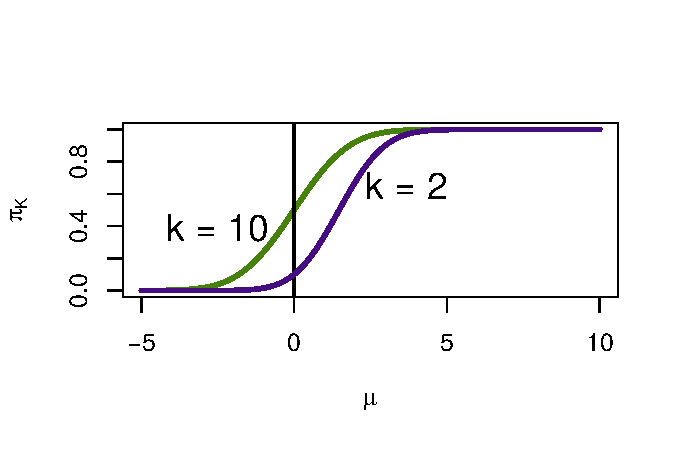
\includegraphics[scale = 0.7, clip=true, trim=0 0.2in 0 0.5in]{Figures/illus_piK_flat_flipped.pdf}
\caption{Left: The function $\pi_k(\mu)$ for $k = \{2, 10\}$.}
\label{fig:pi}
\end{figure}

The estimator we propose is
\begin{equation}\label{eq:hat_i_hd}
\hat{I}_{HD} = \frac{1}{2}(\pi_{k}^{-1}(\text{ABA}_k))^2,
\end{equation}
obtained by inverting the relation \eqref{abepi}, then substituting
an estimate of the identification accuracy $\text{TA}_k$ for the $\text{ABA}_k$.  
%As such,
%our estimator can be directly compared to the $\hat{I}_{Fano}$, since
%both are functions of $\text{ABA}_k$ (Figure \ref{fig:pi}.)

\section{Theory}

\subsection{Assumptions}\label{sec:ch5_assumptions}

The theory applies to a high-dimensional limit where $I(X; Y)$ tends to a constant.

\begin{itemize}
\item[A1.] $\lim_{d \to \infty} I(X^{[d]}; Y^{[d]}) = \iota < \infty.$
\item[A2.] There exists a sequence of scaling constants $a_{ij}^{[d]}$
and $b_{ij}^{[d]}$ such that the random vector $(a_{ij}\ell_{ij}^{[d]} +
b_{ij}^{[d]})_{i, j = 1,\hdots, k}$ converges in distribution to a
multivariate normal distribution,
where $\ell_{ij} = \log p(y^{(i)}|x^{(i)})$ for independent $y^{(i)} \sim p(y|x^{(i)})$.
\item[A3.] Define \[
u^{[d]}(x, y) = \log p^{[d]}(x, y) - \log p^{[d]}(x) - \log p^{[d]}(y).
\]
There exists a sequence of scaling constants $a^{[d]}$, $b^{[d]}$ such that
\[
a^{[d]}u^{[d]}(X^{(1)}, Y^{(2)}) + b^{[d]}
\]
converges in distribution to a univariate normal distribution.
\item[A4.] For all $i \neq k$,
\[\lim_{d \to \infty}\Cov[u^{[d]}(X^{(i)}, Y^{(j)}), u^{[d]}(X^{(k)}, Y^{(j)})] = 0.\]
\end{itemize}

Assumptions A1-A4 are satisfied in a variety of natural models.  One
example is a multivariate Gaussian sequence model where $X \sim N(0,
\Sigma_d)$ and $ Y = X + E $ with $ E \sim N(0, \Sigma_e), $ where
$\Sigma_d$ and $\Sigma_e$ are $d \times d$ covariance matrices, and
where $X$ and $E$ are independent.  Then, if $d \Sigma_d$ and
$\Sigma_e$ have limiting spectra $H$ and $G$ respectively, the joint
densities $p(x, y)$ for $d = 1,\hdots, $ satisfy assumptions A1 - A4.
Another example is the multivariate logistic model, which we describe
in section 3.  We further discuss the rationale behind A1-A4 in the
supplement, along with the detailed proof.

\subsection{Limiting universality}

We obtain the universality result in two steps.  First, we link the
average Bayes error to the moments of some statistics $Z_i$.
Secondly, we use Taylor approximation in order to express $I(X; Y)$ in
terms of the moments of $Z_i$.  Connecting these two pieces yields the
formula \eqref{abepi}.

Let us start by rewriting the average Bayes error:
\[
\text{ABA}_k = \Pr[p(Y|X_1) = \max_{j \neq 1} p(Y|X_j)| X = X_1].
\]
Defining the statistic $Z_i = \log p(Y|X_i) - \log p(Y|X_1)$, where $Y
\sim p(y|X_1)$, we obtain $ e_{ABE} = \Pr[\max_{j > 1} Z_i > 0].  $
The key assumption we need is that $Z_2,\hdots, Z_k$ are
asymptotically multivariate normal.  If so, the following lemma allows
us to obtain a formula for the average Bayes accuracy.

\textbf{Lemma 1. }
\emph{
Suppose $(Z_1, Z_2, \hdots, Z_k)$ are jointly multivariate normal, with 
$\E[Z_1 - Z_i]= \alpha$, 
$\Var(Z_1) = \beta \geq 0$, 
$\Cov(Z_1, Z_i) = \gamma$, 
$\Var(Z_i)= \delta$, and $\Cov(Z_i, Z_j) = \epsilon$ for all $i, j = 2, \hdots,
k$, such that $\beta + \epsilon - 2\gamma > 0$.  Then, letting
\[
\mu = \frac{\E[Z_1 - Z_i]}{\sqrt{\frac{1}{2}\Var(Z_i - Z_j)}} = \frac{\alpha}{\sqrt{\delta - \epsilon}},
\]
\[
\nu^2 = \frac{\Cov(Z_1 -Z_i, Z_1 - Z_j)}{\frac{1}{2}\Var(Z_i - Z_j)} = \frac{\beta + \epsilon - 2\gamma}{\delta - \epsilon},
\]
we have
\begin{align*}
\Pr[Z_1 < \max_{i=2}^k Z_i] &= \Pr[W < M_{k-1}]
\\&= 1 - \int \frac{1}{\sqrt{2\pi\nu^2}} e^{-\frac{(w-\mu)^2}{2\nu^2}} \Phi(w)^{k-1} dw,
\end{align*}
where $W \sim N(\mu, \nu^2)$ and $M_{k-1}$ is the maximum of $k-1$
independent standard normal variates, which are independent of $W$.
}

\emph{Remark.}
To see why the assumption that $Z_2,\hdots, Z_k$ are multivariate
normal might be justified, suppose that $X$ and $Y$ have the same
dimensionality $d$, and that joint density factorizes as
\[
p(x^{(j)}, y) = \prod_{i=1}^d p_i(x^{(j)}_i, y_i)
\]
where $x_i^{(j)}, y_i$ are the $i$th scalar components of the vectors $x^{(j)}$ and $y$.
Then,
\[
Z_i = \sum_{m=1}^d \log p_m(y_m | x^{(i)}_m) - \log p_m(y_m | x^{(m)}_1)
\]
where $x_{i, j}$ is the $i$th component of $x_j$.  The $d$ terms $\log
p_m(y_m | x_{m, i}) - \log p_m(y_m | x_{m, 1})$ are independent across
the indices $m$, but dependent between the $i = 1,\hdots, k$.
Therefore, the multivariate central limit theorem can be applied to
conclude that the vector $(Z_2,\hdots, Z_k)$ can be scaled to converge
to a multivariate normal distribution.  While the componentwise
independence condition is not a realistic assumption, the key property
of multivariate normality of $(Z_2,\hdots, Z_k)$ holds under more
general conditions, and appears reasonable in practice.

\textbf{Proof.}
We can construct independent normal variates $G_1$, $G_2,\hdots, G_k$
such that
\[
G_1 \sim N(0, \beta + \epsilon - 2 \gamma)
\]
\[
G_i \sim N(0, \delta - \epsilon)\text{ for }i > 1
\]
such that
\[
Z_1 - Z_i = \alpha + G_1 + G_i \text{ for }i > 1.
\]
Hence
\begin{align*}
\Pr[Z_1 < \max_{i=2}^k Z_i] &= \Pr[\min_{i > 1} Z_1 - Z_i < 0].
\\&= \Pr[\min_{i=2}^{k} G_1 + G_i + \alpha < 0]
\\&= \Pr[\min_{i=2}^{k} G_i < -\alpha - G_1]
\\&= \Pr[\min_{i=2}^{k} \frac{G_i}{\sqrt{\delta - \epsilon}} < -\frac{\alpha - G_1}{\sqrt{\delta - \epsilon}}].
\end{align*}
Since $\frac{G_i}{\sqrt{\delta - \epsilon}}$ are iid standard normal variates, and since
$-\frac{\alpha - G_1}{\sqrt{\delta - \epsilon}} \sim N(\mu,\nu^2)$ for $\mu$ and $\nu^2$ given in the statement of the Lemma, the proof is completed via a straightforward computation.  $\Box$



It remains to link the moments of $Z_i$ to $I(X;Y)$.  This is accomplished by approximating the logarithmic term by the Taylor expansion
\[
\log \frac{p(x, y)}{p(x) p(y)} \approx \frac{p(x, y) - p(x) p(y)}{p(x) p(y)} - \left(\frac{p(x, y) - p(x) p(y)}{p(x) p(y)}\right)^2 + \hdots.
\]
A number of assumptions are needed to ensure that needed
approximations are sufficiently accurate; and additionally, in order
to apply the central limit theorem, we need to consider a
\emph{limiting sequence} of problems with increasing dimensionality.
We now state the theorem.

\textbf{Theorem 1.} \emph{Let $p^{[d]}(x, y)$ be a sequence of joint densities
for $d = 1,2,\hdots$.  Further assume that
\begin{itemize}
\item[A1.] $\lim_{d \to \infty} I(X^{[d]}; Y^{[d]}) = \iota < \infty.$
\item[A2.] There exists a sequence of scaling constants $a_{ij}^{[d]}$
and $b_{ij}^{[d]}$ such that the random vector $(a_{ij}\ell_{ij}^{[d]} +
b_{ij}^{[d]})_{i, j = 1,\hdots, k}$ converges in distribution to a
multivariate normal distribution,
where $\ell_{ij} = \log p(y^{(i)}|x^{(i)})$ for independent $y^{(i)} \sim p(y|x^{(i)})$.
\item[A3.] Define \[
u^{[d]}(x, y) = \log p^{[d]}(x, y) - \log p^{[d]}(x) - \log p^{[d]}(y).
\]
There exists a sequence of scaling constants $a^{[d]}$, $b^{[d]}$ such that
\[
a^{[d]}u^{[d]}(X^{(1)}, Y^{(2)}) + b^{[d]}
\]
converges in distribution to a univariate normal distribution.
\item[A4.] For all $i \neq k$,
\[\lim_{d \to \infty}\Cov[u^{[d]}(X^{(i)}, Y^{(j)}), u^{[d]}(X^{(k)}, Y^{(j)})] = 0.\]
\end{itemize}
Then for $\text{ABA}_k$ as defined above, we have
\[
\lim_{d \to \infty} \text{ABA}_k = \pi_k(\sqrt{2 \iota})
\]
where
\[
\pi_k(c) = \int_{\mathbb{R}} \phi(z - c)  \Phi(z)^{k-1} dz
\]
where $\phi$ and $\Phi$ are the standard normal density function and
cumulative distribution function, respectively.}


\textbf{Proof.}

For $i = 2,\hdots, k$, define
\[
Z_i = \log p(Y^{(1)}|X^{(i)}) - \log p(Y^{(1)}|X^{(1)}).
\]
Then, we claim that $\vec{Z} = (Z_2,\hdots, Z_k)$ converges in distribution to
\[
\vec{Z} \sim N\left(-2\iota, 
\begin{bmatrix}
4\iota & 2\iota & \cdots & 2\iota\\
2\iota & 4\iota & \cdots & 2\iota\\
\vdots & \vdots & \ddots & \vdots\\
2\iota & 2\iota & \cdots & 4\iota
\end{bmatrix}
\right).
\]
Combining the claim with the lemma (stated below this proof) yields the
desired result.

To prove the claim, it suffices to derive the limiting moments
\[\E[Z_i] \to -2\iota,\]
\[\Var[Z_i] \to 4\iota,\]
\[\Cov[Z_i, Z_j] \to 2\iota,\]
for $i \neq j$,
since then assumption A2 implies the existence of a multivariate normal
limiting distribution with the given moments.

Before deriving the limiting moments, note the following identities.
Let $X' = X^{(2)}$ and $Y = Y^{(1)}$.
\[
\E[e^{u(X', Y)}] = \int p(x) p(y) e^{u(x, y)} dx dy = \int p(x, y) dx dy = 1.
\]
Therefore, from assumption A3 and the formula for gaussian exponential
moments, we have
\[
\lim_{d \to \infty} \E[u(X', Y)]-\frac{1}{2}\Var[u(X', Y)] = 0.
\]
Let $\sigma^2 = \lim_{d \to \infty} \Var[u(X', Y)]$.
Meanwhile, by applying assumption A2,
\begin{align*}
\lim_{d \to \infty} I(X; Y) &= \lim_{d \to \infty} \int p(x, y) u(x, y) dx dy 
= \lim_{d \to \infty} \int p(x) p(y) e^{u(x, y)} u(x, y) dx dy
\\&= \lim_{d \to \infty}  \E[e^{u(X, Y')}u(X, Y')]
\\&= \int_{\mathbb{R}} e^z z \frac{1}{\sqrt{2\pi \sigma^2}} 
e^{-\frac{(z + \sigma^2/2)^2}{2\sigma^2}} \text{ (applying A2)}
\\&= \int_{\mathbb{R}} z \frac{1}{\sqrt{2\pi \sigma^2}} 
e^{-\frac{(z - \sigma^2/2)^2}{2\sigma^2}}
\\&= \frac{1}{2}\sigma^2.
\end{align*}
Therefore,
\[
\sigma^2 = 2\iota,
\]
and
\[
\lim_{d \to \infty} \E[u(X', Y)] = -\iota.
\]
Once again by applying A2, we get
\begin{align*}
\lim_{d \to \infty} \Var[u(X, Y)] 
&= \lim_{d \to \infty} \int (u(x, y) - \iota)^2 p(x, y) dx dy
\\&= \lim_{d \to \infty} \int (u(x, y) - \iota)^2 e^{u(x, y)} p(x) p(y) dx dy
\\&= \lim_{d \to \infty} \E[(u(X', Y) - \iota)^2 e^{u(X', Y)}] 
\\&= \int (z - \iota)^2 e^z \frac{1}{\sqrt{4\pi\iota}} e^{-\frac{(z+\iota)^2}{4\iota}} dz \text{ (applying A2)}
\\&= \int (z - \iota)^2 \frac{1}{\sqrt{4\pi\iota}} e^{-\frac{(z-\iota)^2}{4\iota}} dz
\\&= 2\iota.
\end{align*}


We now proceed to derive the limiting moments.
We have
\begin{align*}
\lim_{d \to \infty} \E[Z] 
&= \lim_{d \to \infty} \E[ \log p(Y|X') - \log p(Y|X)]
\\&= \lim_{d \to \infty} \E[ u(X', Y) - u(X, Y) ] = -2\iota.
\end{align*}
Also,
\begin{align*}
\lim_{d \to \infty} \Var[Z]
 &= \lim_{d \to \infty} \Var[ u(X', Y) - u(X, Y) ]
\\&= \lim_{d \to \infty} \Var[ u(X', Y)] +\Var[ u(X, Y) ]\text{ (using assumption A4) }
\\&= 4\iota,
\end{align*}
and similarly
\begin{align*}
\lim_{d \to \infty} \Cov[Z_i, Z_j]
&= \lim_{d \to \infty} \Var[ u(X, Y)]\text{ (using assumption A4) }
\\&= 2\iota.
\end{align*}
This concludes the proof. $\Box$.

\section{Examples}

We demonstrate the application of our proposed estimators,
$\hat{I}_{Ident}$, which was introduced in the previous chapter, and
the estimator $\hat{I}_{HD}$ based on high-dimensional asymptotics, as
defined in \eqref{eq:hat_i_hd}.

We compare our methods to a number of existing methods for mutual
information.  For any $k$-class classification task, define the $k
\times k$ \emph{confusion matrix} $M$ as the matrix whose $i, j$
counts how many times a output in the $i$th class was classified to
the $j$th class.

The estimator $\hat{I}_{Fano}$ is based on Fano's inequality, which reads
\[
H(Z|Y) \leq H(1-\text{BA}) + (1-\text{BA}) \log ||\mathcal{Z}| - 1|
\]
where $\text{BA}$ is Bayes accuracy, and $H(e)$ is the entropy of a
Bernoulli random variable with probability $e$.  Replacing $H(Z|Y)$
with $H(X|Y)$ and replacing $\text{BA}$ with the test accuracy $\text{TA}$,
we get the estimator
\[
\hat{I}_{Fano} = log(K) - (1-\text{TA}) log(K-1) + (1-\text{TA}) log(1-\text{TA}) + \text{TA} log(\text{TA}).
\]
Meanwhile, the confusion matrix estimator computes
\[
\hat{I}_{CM} = \frac{1}{k^2} \sum_{i=1}^k \sum_{j=1}^k \log \frac{M_{ij}}{r/k},
\]
which is the empirical mutual information of the discrete joint
distribution $(Z, f(Y))$.

The estimator $\hat{I}_0$ is the so-called `naive' estimate of mutual information, based on the identity
\[
I(X;Y) = H(Y) - H(Y|X).
\]
Given any nonparametric estimator of entropy $\hat{H}$, we obtain
\[
\hat{I}_0 = \hat{H}(Y) - \sum_{i=1}^k \hat{H}(Y|X^{(i)}).
\]
We use the polynomial-based entropy estimator introduced by
\cite{jiao2015minimax} as the estimator of entropy.  

It is known that $\hat{I}_0$ tends to underestimate the mutual
information.  Therefore, Gastpar et al. introduced the anthropic
correction estimator $\hat{I}_\alpha$ which adds a bias-correction
term \footnote{However, without a principled approach to choose the
  parameter $\alpha \in (0,1]$, $\hat{I}_\alpha$ could still vastly
underestimate or overestimate the mutual information.}to $\hat{I}_0$.

\subsection{Simulation}

We compare the estimators $\hat{I}_{CM}$, $\hat{I}_{Fano}$,
$\hat{I}_{HD}$ with a nonparametric estimator $\hat{I}_\alpha$
(\cite{Gastpar2009}) in the following simulation, and the correctly
specified parametric estimator $\hat{I}_{MLE}$.  We generate data
according to a multiple-response logistic regression model, where $ X
\sim N(0, I_p) $, and $Y$ is a binary vector with conditional
distribution
\[
Y_i|X = x \sim \text{Bernoulli}(x^T B_i)
\]
where $B$ is a $p \times q$ matrix.  We generate training data with
$r$ responses per stimulus $X^{(i)}$.  One application of this model
might be modeling neural spike count data $Y$ arising in response to
environmental stimuli $X$ (\cite{banerjee2012parametric}).  We choose
the naive Bayes for the classifier $\mathcal{F}$: it is consistent for
estimating the Bayes rule.

\begin{figure}
\centering
\begin{tabular}{cc}
a & b\\
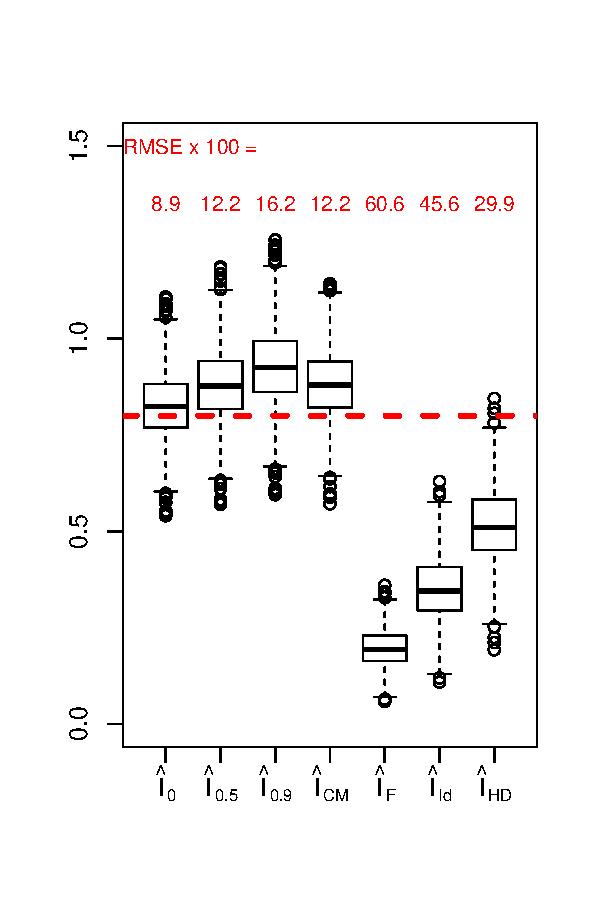
\includegraphics[scale = 0.5]{../../info_theory_sims/fig1_with_Id.pdf} &
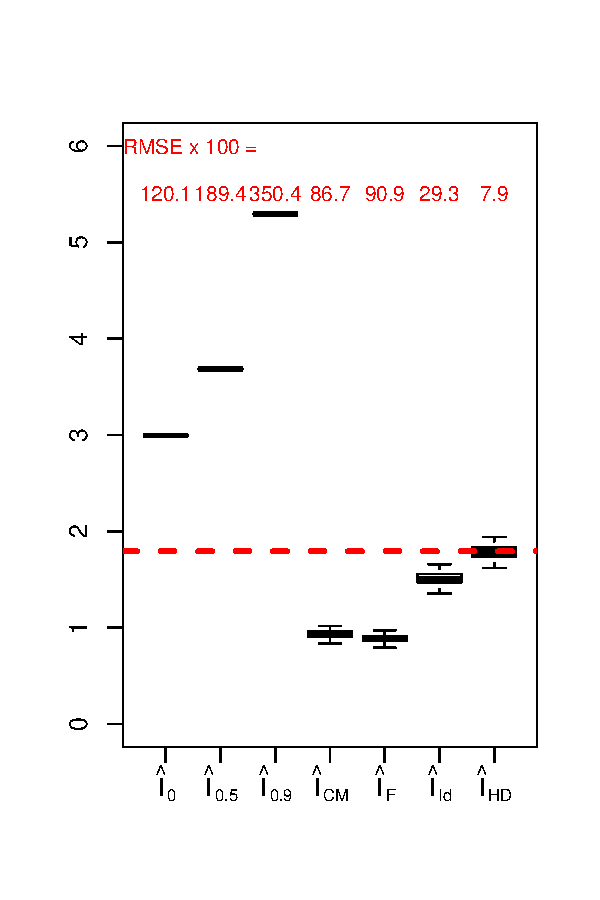
\includegraphics[scale = 0.5]{../../info_theory_sims/fig2_with_Id.pdf}
\end{tabular}
\caption{Simulation for inferring mutual information in a gaussian random classification model}
\label{fig:gaussian_sim}
\end{figure}

Figure \ref{fig:gaussian_sim} displays the simulation results for two
cases: 
\begin{itemize}
\item[(a).] A low-dimensional example with $\{p = 3$, $q = 3$, $B = \frac{4}{\sqrt{3}} I_3$, $K = 20$, $r = 40\}$
\item[(b).] A high-dimensional example with $\{p = 50$, $q = 50$, $B = \frac{4}{\sqrt{50}} I_{50}$, $K = 20$, $r = 8000\}$
\end{itemize}
We see that in the low-dimensional example, the na\"{i}ve estimator
$\hat{I}_0$ achieves the best performance, with both of our proposed
estimators $\hat{I}_{Ident}$ and $\hat{I}_{HD}$ biased downwards.
However, in the high-dimensional example, which approximately
satisfies the assumptions of our high-dimensional theory, we see that
all estimators of mutual information become highly concentrated.
Therefore, it is the amount of bias in the estimator that mainly
determines estimation performance.  We see heavy bias in estimators
except for $\hat{I}_{HD}$, which is to be expected since the
nonparametric estimators $\hat{I}_\alpha$ scale poorly in high
dimensions, while $\hat{I}_{CM}, \hat{I}_{Fano}$ and $\hat{I}_{Ident}$
are based on lower bounds and therefore should have a downward bias.

\subsection{Real data example}\label{sec:real_data}

\cite{Kay2008a} employed a randomized stimuli design in their 2008 paper,
``Identifying Natural Images from Human Brain Activity.''  The
experiment was designed in order to investigate how visual information
from natural images is encoded in the V1 through V3 brain regions.
The stimulus space, $\mathcal{X}$, consists of $128 \times 128$-pixel
grayscale photographs.  The response data consists of BOLD response in
regions V1, V2, and V3 from a single subject.  The raw time series were
processed to yield a single averaged response vector $y^{(i)}$ for each
stimulus $x^{(i)}$, for $i = 1,\hdots, 1870$.
The dimensionality of $y^{(i)}$ varies depending on which regions of interest
we are discussing, and whether we consider a subset of the voxels in those regions.
Let $v$ denote the dimensionality (number of voxels) of $y$.

Let $x^{(i)}$ denote the native $128 \times 128$-pixel representation
of the image (i.e. a $16384$-dimensional vector with entries between 0
and 1.)  One of the goals of the Kay et al. paper is to evaluate
competing encoding models.  In the context of the study,
an \emph{encoding model} is a vector-valued function from the stimulus
to a $p$-dimensional space,
\[
\vec{g}(x) = (g_1(x),\hdots, g_{p}(x)).
\]
One of the encoding models studied by Kay et al. is the Gabor wavelet pyramid,
$\vec{g}_{Gabor}$, with $p = 10921$.
Using a \emph{training} subset of the stimulus-response pairs $(x_i, y_i)$, $i = 1,\hdots, 1750$,
Kay et al. fit a regularized linear model
\[
y^{(i)} \approx B^T \vec{g}(x^{(i)})
\]
where $B$ is a $10921 \times v$-dimensional matrix, which is to be fit
to the data.  Then they computed the identification accuracy for $k$
(number of stimulus classes) ranging from 2 to 1000.

Using the Kay et al. data, we sort voxels in V1 according to estimated
signal-to-noise ratio (\cite{benjamini2013shuffle}).  Then, using
cross-validated elastic net on the top $p = \{100, 200, 300, 400,
500\}$ voxels, we compute the identification accuracy for $k =
\{20,\hdots, 240\}$ classes.  The test identification accuracy was
used to estimate mutual information using both $\hat{I}_{Ident}$ and
$\hat{I}_{HD}$.  Due to the dimensionality of the data, we expected
$\hat{I}_{HD}$ to yield more accurate estimates of mutual information.

The estimated mutual information using $k = 240$ is displayed in
Figure \ref{fig:n_voxels_vs_mi}.  Both estimators indicate a large
jump in the mutual information when going from 100 to 200 voxels,
almost no increase from 200 to 400, then a slight increase in
information from 400 to 500.  The two estimators $\hat{I}_{Ident}$ and
$\hat{I}_{HD}$ differ significantly for all numbers of voxels. We see
from this that it is important to choose the estimator which is best
suited for the application: if the high-dimensional assumption can be
justified, $\hat{I}_{HD}$ can yield a much better estimate; but if not
justified, then it could be a significant overestimate of the mutual
information, and it would be preferable to use $\hat{I}_{Ident}$.

\begin{figure}
\centering
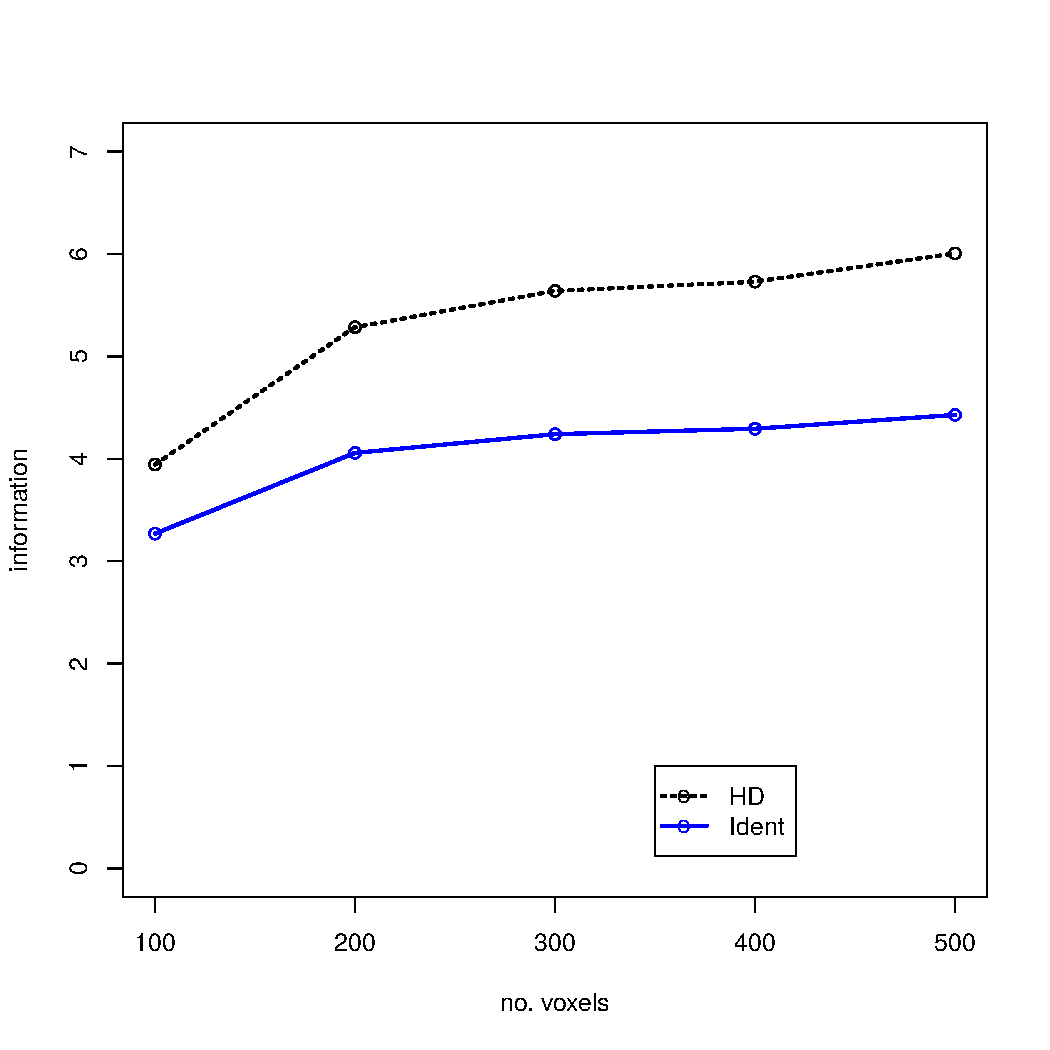
\includegraphics[scale = 0.5]{../../Yuval/info_infer_edited.pdf}
\caption{Estimated mutual information for different subsets of V1 voxels}
\label{fig:n_voxels_vs_mi}
\end{figure}

Next, let us examine the sensitivity of the point estimates to the
choice of the tuning parameter $k$.  Figure \ref{fig:dependence_k}
shows how the estimates displayed in the previous figure depend on the
choice of $k$.  For all numbers of voxels, we see that $k$ does have
an appreciable affect on the resulting estimate of mutual information.
This is predicted from the theory for $\hat{I}_{Ident}$, but under the
high-dimensionality assumptions $\hat{I}_{HD}$ should not
significantly depend on $k$.  Therefore, the sensitivity of
$\hat{I}_{HD}$ we see, especially for the 500-voxel case, indicates a
detectable violation of the asymptotic assumptions.

Given such evidence for violation of assumptions, the conservative
approach would be to abandon $\hat{I}_{HD}$ in this situation and
choose $\hat{I}_{Ident}$ as the estimator. Since $\hat{I}_{Ident}$ is
an underestimate for all $k$, one should choose the $k$ which
maximizes the estimated mutual information.  However, even then, as we
see from the earlier simulation, we can expect $\hat{I}_{Ident}$ to
significantly underestimate the true mutual information.

\begin{figure}
\centering
\begin{tabular}{cc}
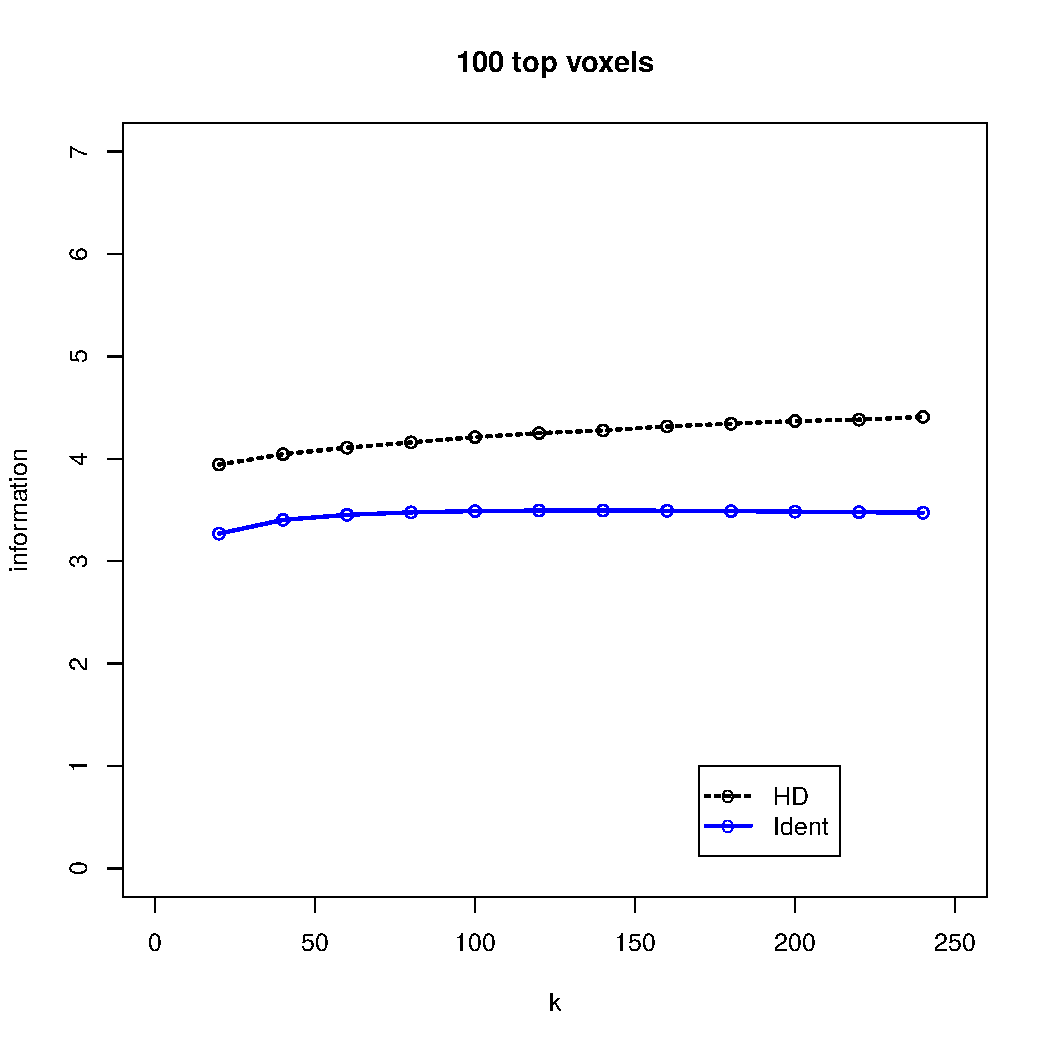
\includegraphics[scale = 0.4]{../../Yuval/ident_infer1_edited.pdf} &
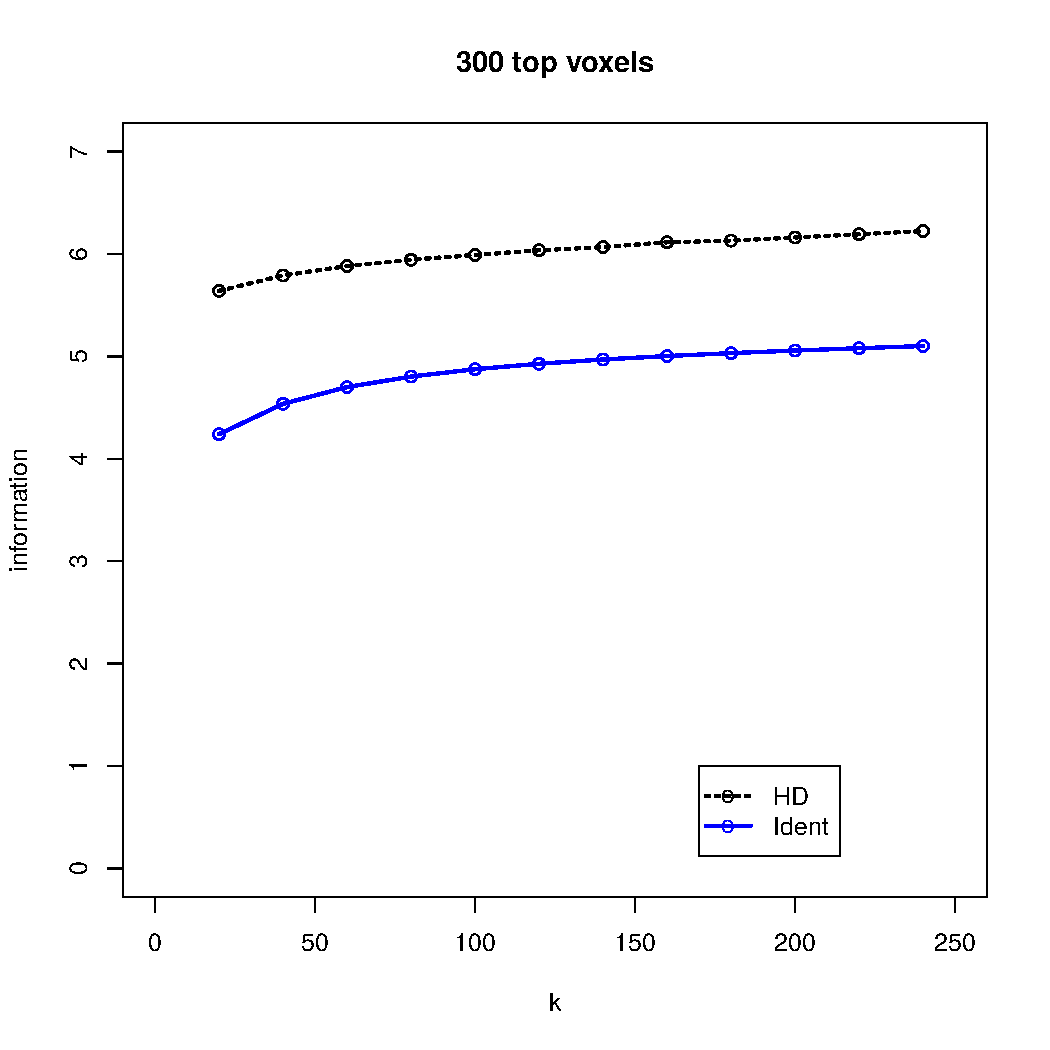
\includegraphics[scale = 0.4]{../../Yuval/ident_infer3_edited.pdf} \\
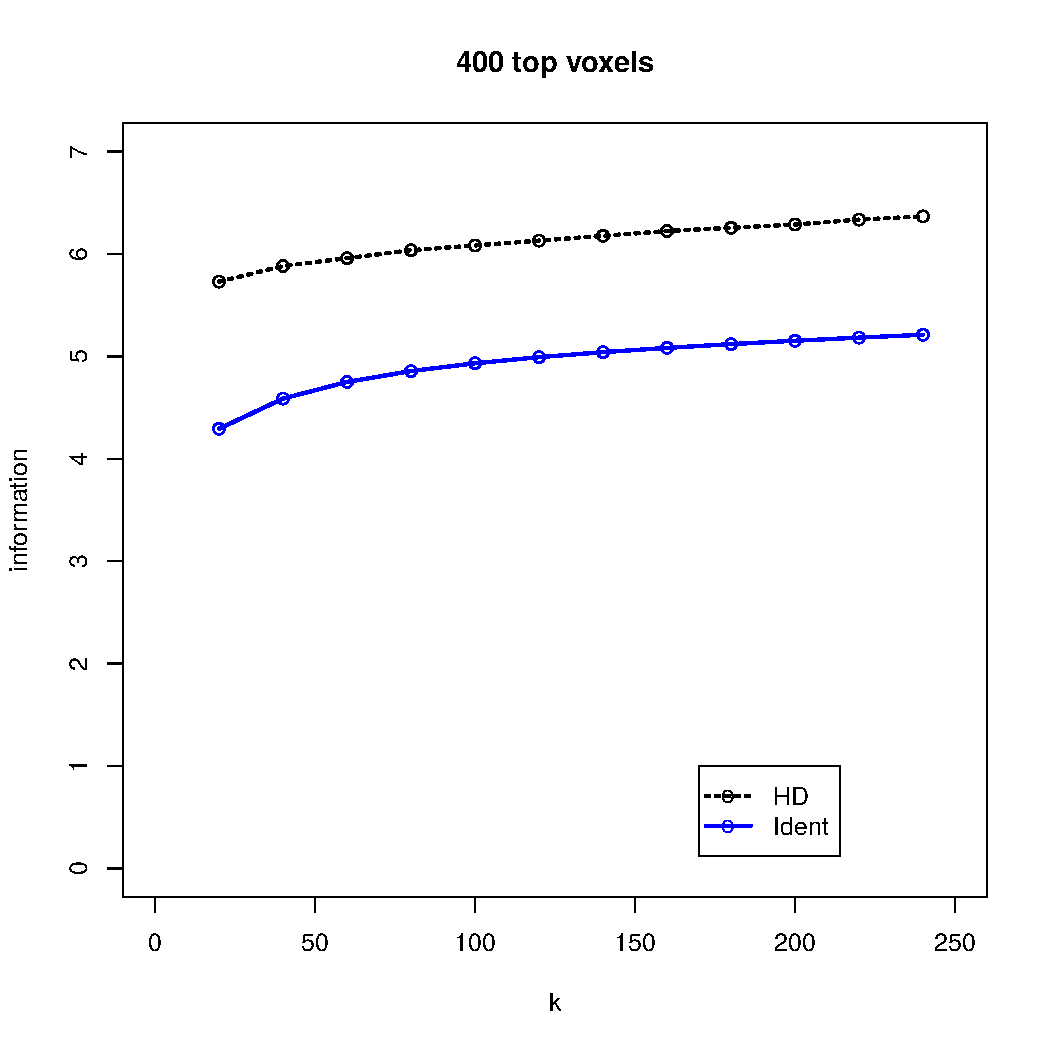
\includegraphics[scale = 0.4]{../../Yuval/ident_infer4_edited.pdf} &
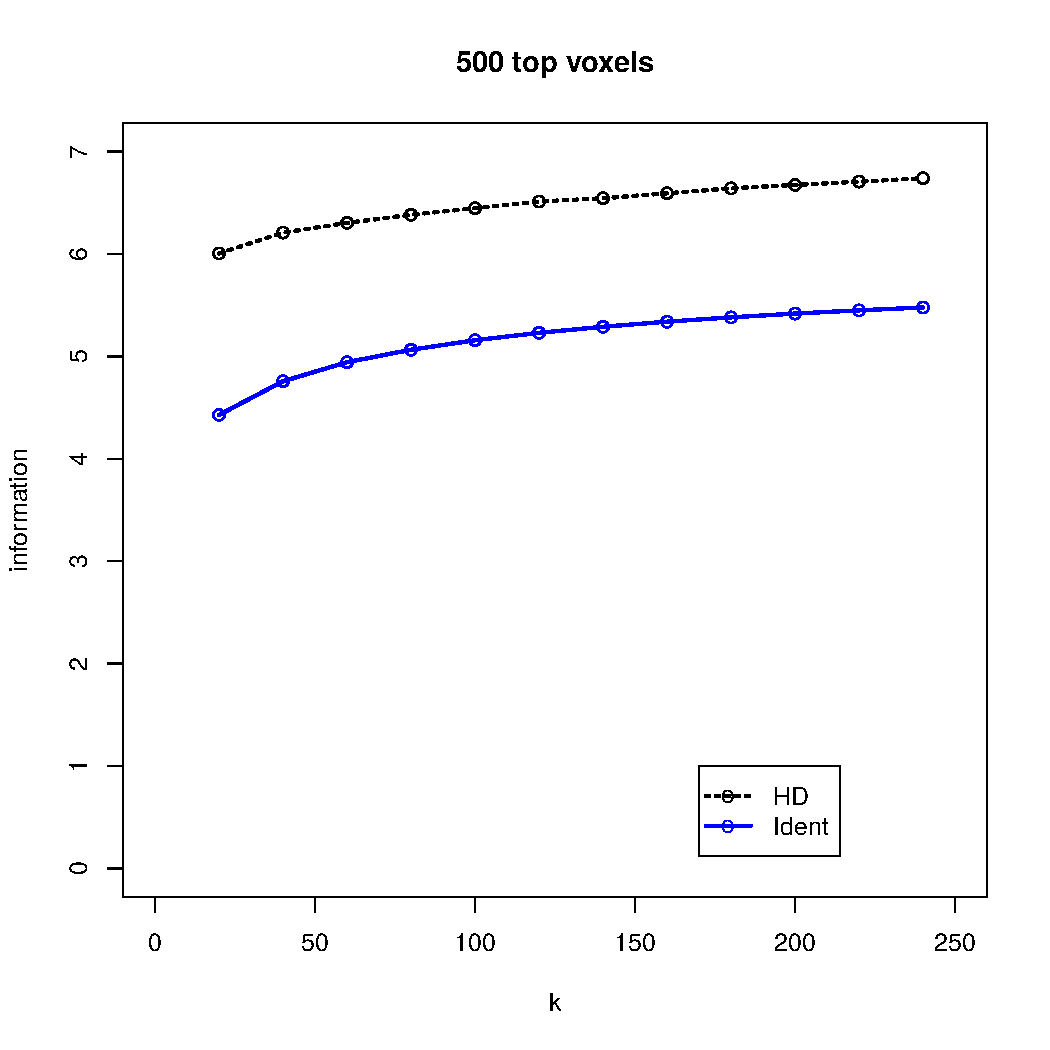
\includegraphics[scale = 0.4]{../../Yuval/ident_infer5_edited.pdf}
\end{tabular}
\caption{Dependence of estimated mutual information on $k$}
\label{fig:dependence_k}
\end{figure}


